\subsection{Organisation d'une application basée sur une telle architecture}
\paragraph{}
Dans une application, les besoins fonctionnels et non fonctionnels peuvent être différents selon que l'on s'intéresse à ses composantes de lecture ou d'écriture.
Dans le cas d'une IHM, il est important que l'information que l'on souhaite afficher soit disponible à l'utilisateur sans qu'il n'ait à croiser lui-même différentes informations présentes sur différents écrans.
Il est alors nécessaire d'aggréger et de filtrer les données et donc de les dénormaliser lorsqu'elles sont destinées à la consultation.
D'autre part, lorsqu'un utilisateur souhaitera exécuter une action d'écriture, l'ensemble des données manipulées sera plus réduit et la problématique ne sera plus la même.
La complexité se trouvera plutôt dans la vérification du respect de règles et il sera nécessaire d'utiliser des entités d'association pour ce faire.
Ainsi, on privilégie dans ce cas une normalisation des données ainsi que leur intégrité.
On voit alors que les besoins en écriture sont globalement transactionnels et une garantie de cohérence des données ainsi que leur normalisation est nécessaire, tandis qu'en lecture, les besoins sont davantage en dénormalisation des données ainsi qu'en scalabilité.
\paragraph{}
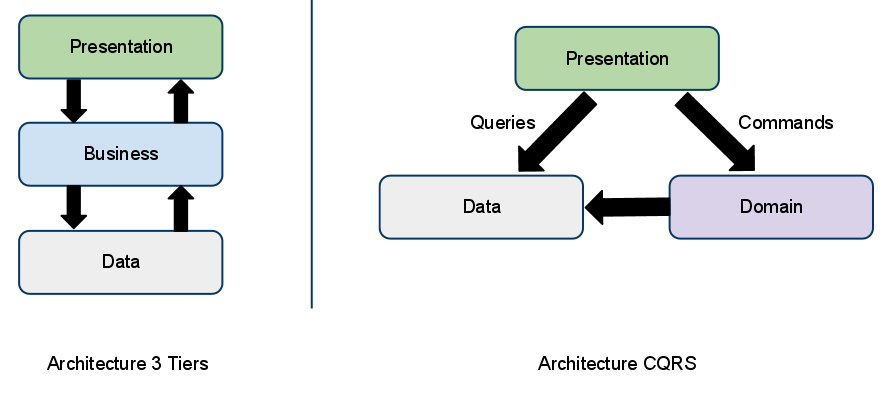
\includegraphics[scale=0.4]{Figures/Chapter3/architecture/tiersvscqrs.png}
Par opposition à une architecture du type 3 tiers, dont les services permettant d'accéder aux données se confondent avec ceux qui vont agir sur ces même données, l'architecture CQRS sépare volontairement les composants requêtant les données de ceux qui les modifient.
Une telle séparation facilite l'organisation de l'application puisque des composants différents sont utilisés pour des problématiques différentes, mais permet aussi de profiter des avantages de différentes technologies sur ces composants et ainsi d'optimiser les performances de l'application.
On peut ainsi découper l'architecture du modèle CQRS en différentes couches.

%-------------------------------------------------------------------------
\subsubsection{La couche de modification des données: Command}
\label{subs:La couche de modification des données: Command}
\paragraph{}
Cette couche concentre toutes les modifications des données, qu'il s'agisse de création, de suppression ou de mise à jour.
Une commande représente une action destinée à être exécutée, une intention, et n'est pas une simple demande d'altération de donnée.
Généralement, une commande est représentée comme un appel de méthode encapsulée dans un objet; elle porte un nom explicite et ses champs contiennent les différents paramètres de l'action.
Dans le cas de l'espace recruteur du site Cadremploi.fr, les commandes ont pour but d'enregistrer les altérations effectuées par les événements côté client, et on retrouve des commandes nommées 'ModifierTitrePosteCommand' ou 'PayerOffreCommand' par exemple, permettant de modifier le titre du poste dans l'annonce ou de payer l'offre saisie respectivement.
De tels noms sont ainsi très expressifs et permettent de clarifier la cause de la modification des données.
\paragraph{}
Les méthodes de commandes prennent ainsi en paramètre des identifiants d'entités ainsi que des valeurs simples, ne renvoient rien mais peuvent générer des exceptions.
Ces restrictions assurent que les données manipulées restent légères et que l'action exécutée ne gère que de l'écriture.

%-------------------------------------------------------------------------
\subsubsection{Le domaine}
\label{subs:Le domaine}
Le domaine est la zone où est concentré toute la connaissance métier de l'application.
C'est notamment de là que chaque commande est analysée et qu'il est décidé si l'on donne suite à chacune d'entre elle.
\paragraph{}
Contrètement, les commandes ont accès au domaine via des objets de type Repository.
Ce sont des objets que l'on retrouve en Domain Driven Design (DDD) servant d'intermédiaires entre \ref(subs:Le domaine){le domaine} et la base de donnée.
Ces Repositories permettent d'obtenir l'entitée visée par la commande.
Via les informations contenues dans cette entitées et potentiellement avec différents services, les contrôles nécessaires à la validation d'une commande peuvent être appliqués.
Une fois que les différents contrôles sur les commandes faits, on applique son effet.
Cela permet de maîtriser l'impact de chaque action sur le système.

%-------------------------------------------------------------------------
\subsubsection{La couche de lecture des données: Query}
\label{subs:La couche de lecture des données: Query}
\paragraph{}
La partie Query de ce modèle se base sur le fait que les objets du \ref(subs:Le domaine){domaine} sont volumineux et qu'il est possible de s'en passer.
Cette couche fonctionne ainsi uniquement en lecture seule et aucune modification n'est apportée aux données.
En effet le besoin représenté ici est celui d'une lecture dans un cas d'utilisation bien précis, l'objectif est d'aller extrêmement vite.
Le pattern Query consiste alors à exécuter une requête précise en base et de restituer un objet de type Data Transfer Object (DTO) concis qui pourra être utilisé directement.
Cela signifie que les contrôles sont réduits au minimum et que les DTOs utilisés sont des objets représentant exactement et uniquement le besoin en lecture, généralement des besoins IHM.
Cette méthode permet de récupérer seulement les données dont on a besoin en une fois, en se passant ainsi de parcourir plusieurs tables à travers desquelles les données seraient éparpillées.

\paragraph{}
\label{par:Organisation conclusion}
L'architecture CQRS possède plusieurs avantages

%-------------------------------------------------------------------------
\subsubsection{Les events}
\label{subs:Les events}
Les événements sont des objets stockés dans ce que l'on appelle l'Event Store.
Chaque événement porte une information relative à un changement d'état du système.
Il est ainsi possible de retrouver tout état dans lequel le système a été grâce à un stockage ordonné des événements.
Les événements stockés dans l'Event Store sont également publiés dans un bus de manière à être traités par les Event Handler, dont le rôle est de répercuter sur le système les changements demandés par chaque événement.
La publication d'événements dans ce bus permet de découpler la partie lecture de la partie écriture du système puisqu'il permet de mettre à jour les projections de la partie de lecture sans impacter le domaine.
En effet, l'événement porte ainsi l'information que l'état de l'application a évolué et qu'un changement doit donc être pris en compte dans la partie lecture.
